\chapter{\chapternamedatabase}\label{cap:database}

Neste capítulo, apresentamos os dados utilizados neste trabalho, incluindo as fontes de dados fotométricos. Os dados espectroscópicos serão apresentados e discutidos no apêndice \ref{chap:spectra} e no capítulo \ref{chap:spectra_emission}. 

Primeiramente, descrevemos o levantamento \ac{splus}, suas características e os dados obtidos. Em seguida, detalhamos os procedimentos de correção de extinção aplicados às magnitudes fotométricas. Apresentamos também como os dados foram selecionados para a análise, incluindo os parâmetros utilizados para a fotometria e a seleção de galáxias, magnitudes limites e flags de qualidade.

\section{S-PLUS}
O \ac{splus}, um levantamento do céu do hemisfério sul, localizado no Cerro Tololo Inter-American Observatory, Chile (CTIO), tem como objetivo observar uma área de 9300 graus quadrados do céu com o telescópio robótico de 80 cm T80-South \citep{oliveira2019splus}. Ele disponibiliza 12 filtros fotométricos (Figura \ref{splus_filters}), sendo 5 de banda larga ($u$, $g$, $r$, $z$) e 7 de banda estreita (J0378, J0395, J0410, J0430, J0515, J0660 e J0861).

\begin{figure}[!ht]
    \begin{center}
    % \setcaptionmargin{1cm}
    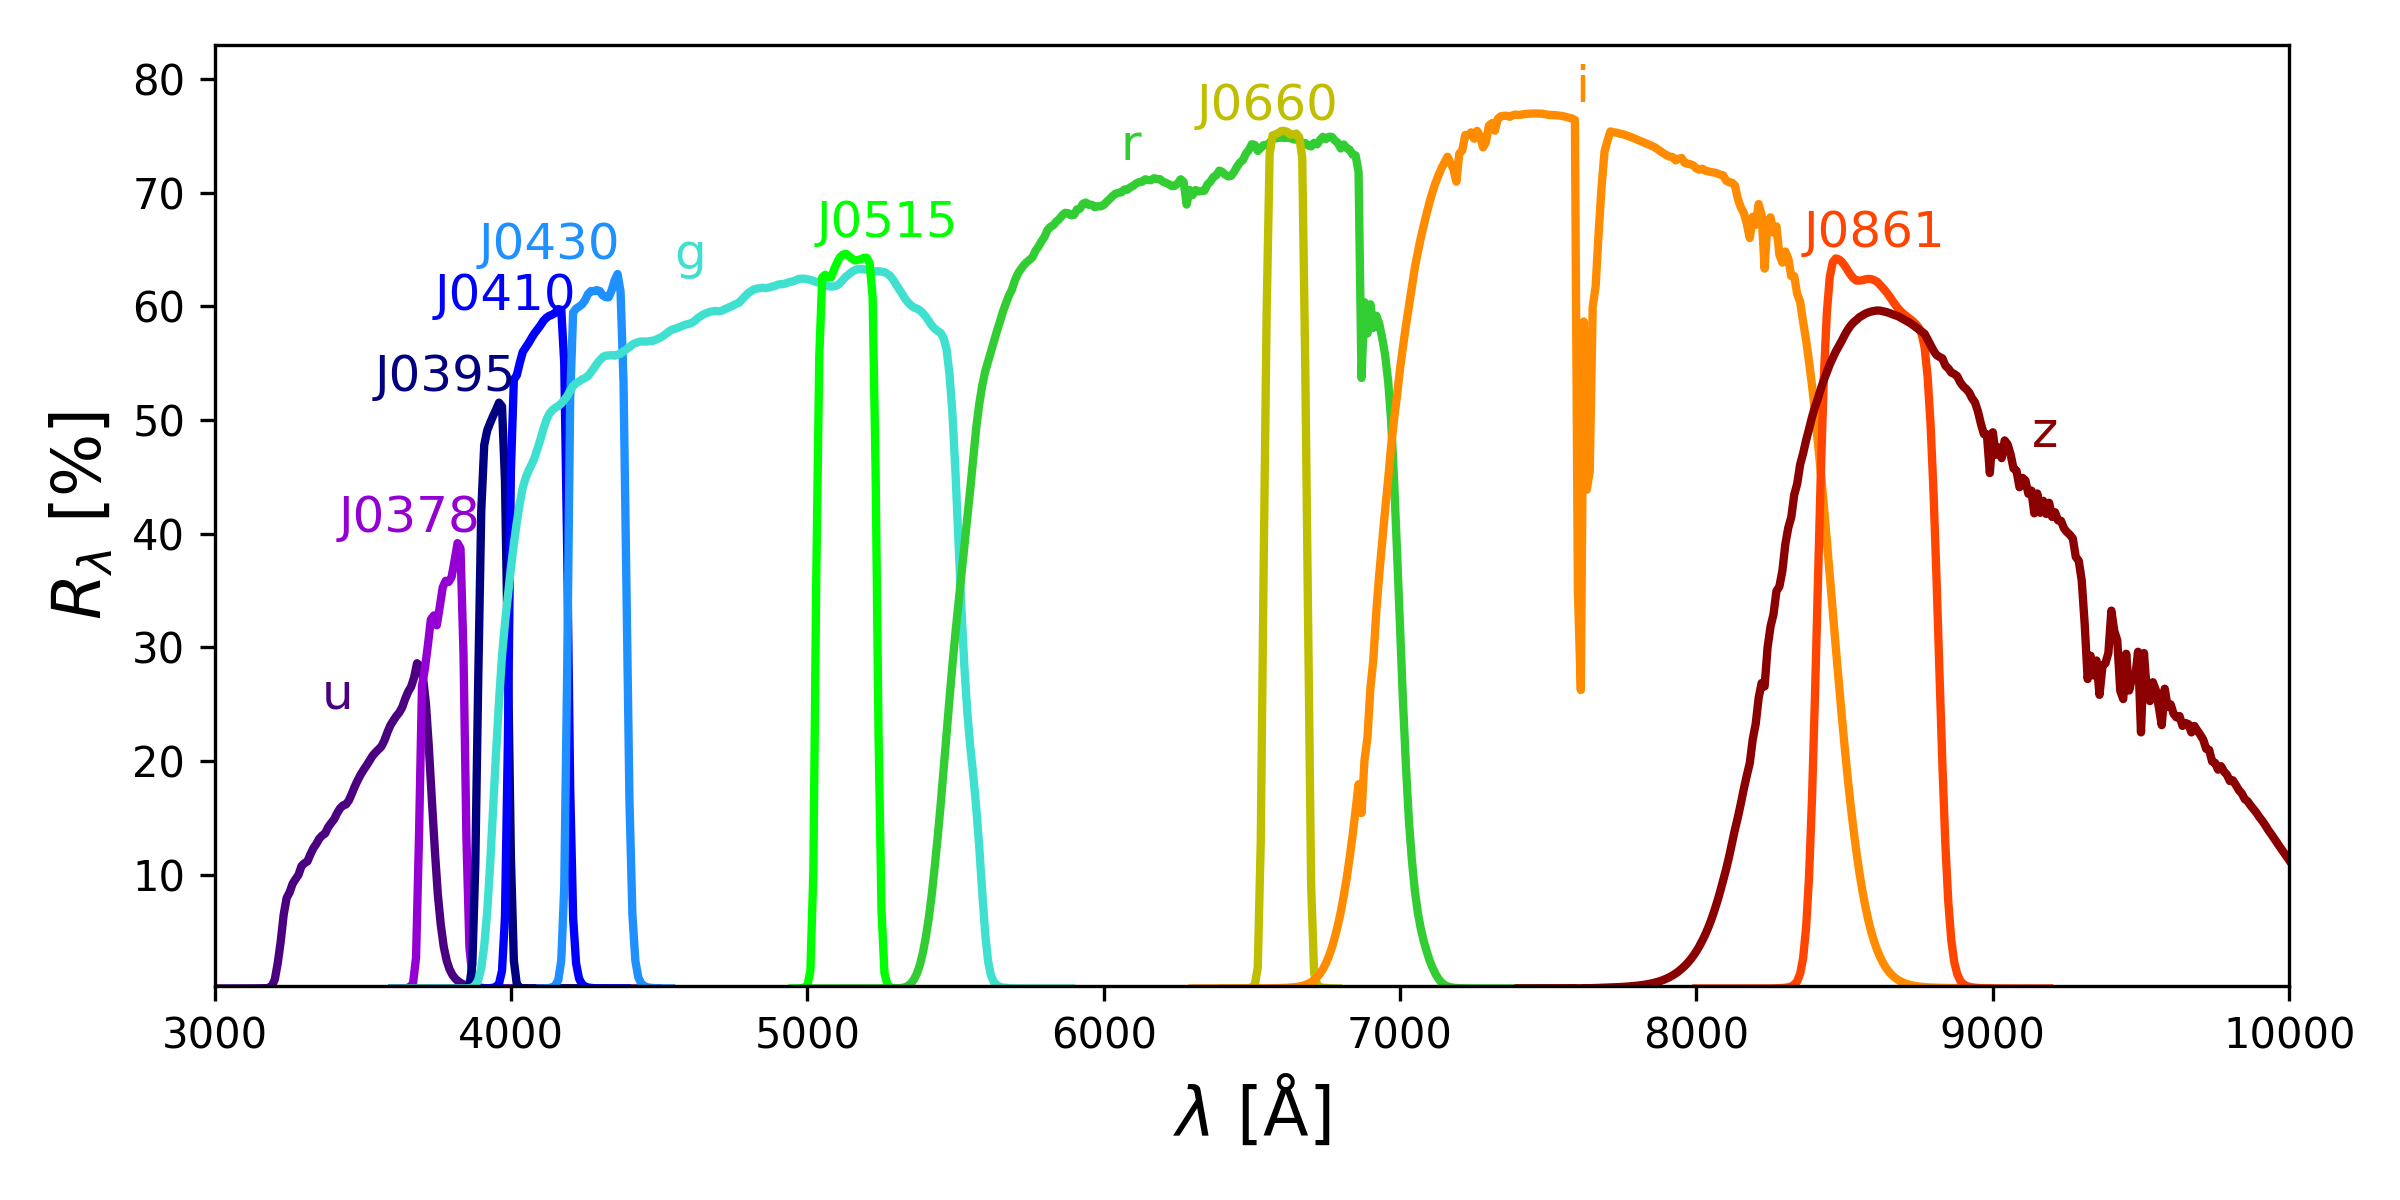
\includegraphics[width=1.0 \columnwidth,angle=0]{splus_filters.png}
    \caption[]{Curvas de resposta dos 12 filtros fotométricos do S-PLUS \citep{splus_DR4_footprint}.}
    \label{splus_filters}
    \end{center}
\end{figure}

Os dados utilizados neste trabalho foram obtidos a partir do quarto lançamento de dados do S-PLUS (\ac{DR4}) \citep{herpich2024fourthsplusdatarelease}. O DR4 cobre uma área de 3022,7 graus quadrados, composta por 1629 campos, cada um deles com um campo de visão de aproximadamente 2 graus quadrados. A Figura \ref{footprint_iDR4} mostra a área coberta pelo S-PLUS \ac{DR4}.

\begin{figure}[!ht]
    \begin{center}
    % \setcaptionmargin{1cm}
    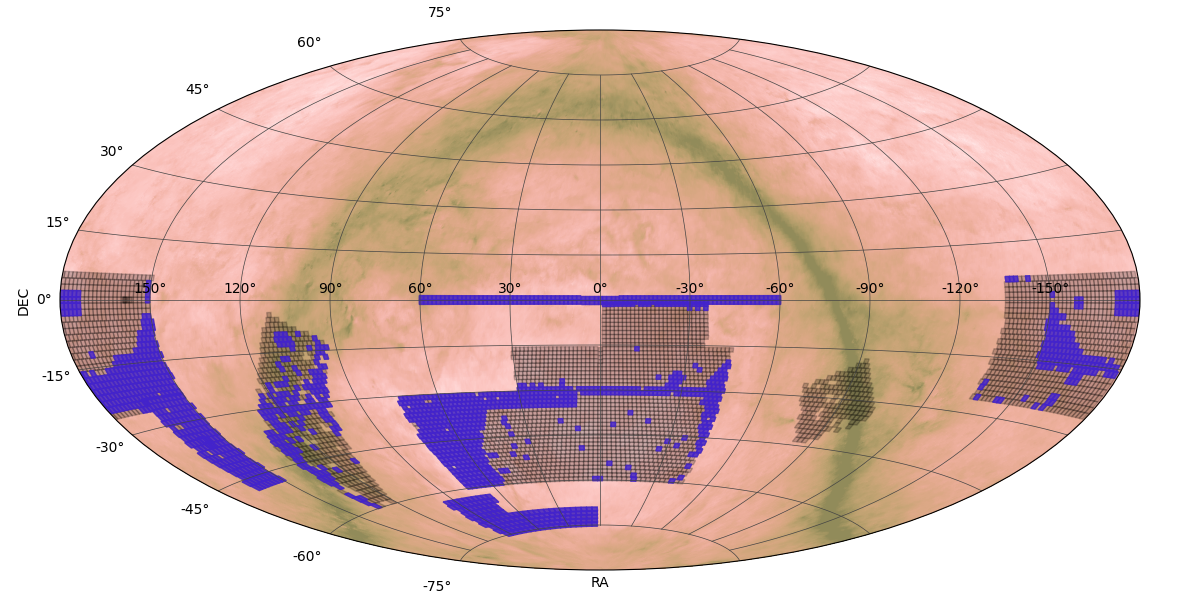
\includegraphics[width=1.0 \columnwidth,angle=0]{footprint_iDR4.png}
    \caption[]{Área coberta pelo S-PLUS DR4. Campos em azul são os observados até o DR4.}
    \label{footprint_iDR4}
    \end{center}
\end{figure}

Além dos 12 filtros fotométricos mencionados, temos opções dos tipos de magnitudes para cada uma dessas bandas. Entre os tipos de magnitudes disponíveis, destacam-se:

\begin{itemize}
    \item \textbf{ISO}: Captura o fluxo dentro de uma isofota, definida por um limite de brilho superficial constante.
    \item \textbf{PETRO}: Mede o fluxo utilizando a abertura de Petrosian, que captura uma fração constante da luz total da galáxia, minimizando a perda de luz nas regiões externas.
    \item \textbf{AUTO}: Abertura adaptativa que utiliza um algoritmo automático para ajustar a abertura ao tamanho e forma do objeto.
    \item \textbf{APER\_3}: Abertura fixa de 3 pixels de raio, adequada para medir o fluxo em regiões centrais.
    \item \textbf{APER\_6}: Abertura fixa de 6 pixels de raio, usada para capturar uma área maior do objeto, balanceando entre evitar contaminação de fontes próximas e capturar mais do fluxo total.
\end{itemize}

Para este trabalho, escolhemos utilizar as magnitudes baseadas na abertura APER\_6. A escolha foi motivada pela necessidade de uma medida consistente para os objetos mais compactos, como as galáxias ultracompactas (UCDs) que estamos buscando.

\subsection{Fotometria de Fornax}\label{sec:Fornax_data}
Os dados do aglomerado de Fornax foram obtidos a partir da mesma fonte que os dados do S-PLUS, o DR4. É importante ressaltar que tanto a fotometria do DR4 quanto as magnitudes de \cite{haack2024splusfornaxprojectsfp} não são corrigidas por extinção interestelar. A partir da colaboração descrita em \cite{castelli2024splusfornaxprojectsfp}, utilizamos a fotometria de \cite{haack2024splusfornaxprojectsfp}, onde foram realizadas novas execuções específicas do \ac{SExtractor} (SExtractor) no DR4, identificando o conjunto mais adequado de parâmetros para recuperar o máximo possível de galáxias de Fornax com fotometria confiável e evitando duplicações.

Os parâmetros da RUN 1 de \cite{haack2024splusfornaxprojectsfp} foram projetados para identificar galáxias fracas e objetos compactos próximos a galáxias mais brilhantes. Por outro lado, os parâmetros da RUN 2 são voltados para uma boa caracterização de galáxias brilhantes e extensas. Assim, para detectar objetos compactos como anãs ultra-compactas (UCDs) ou aglomerados globulares (GCs) perto das galáxias de Fornax, os parâmetros da RUN 1 são mais adequados. Já para caracterizar melhor os objetos mais brilhantes e extensos em Fornax, os parâmetros da RUN 2 são mais eficazes. No nosso caso, usamos os dados da RUN 1. Assim, todos as magnitudes e parâmetros dos \ac{SExtractor} que usamos ao longo do trabalho são da RUN 1 de \cite{haack2024splusfornaxprojectsfp}.

A superioridade da RUN 1 na detecção de UCDs e GCs, em comparação com a configuração padrão do DR4 do SExtractor, advém de parâmetros configurados para otimizar a detecção de objetos compactos e tênues. A RUN 1 emprega um \textit{DEBLEND\_MINCONT} mais elevado (0.005, contra 0.0002 no DR4), tornando-a menos propensa a fragmentar objetos próximos e permitindo que as UCDs sejam detectadas como entidades únicas, mesmo nas proximidades de galáxias mais brilhantes. Além disso, um \textit{DEBLEND\_NTHRESH} menor (32, contra 64 no DR4) e um \textit{BACK\_SIZE} reduzido (64, contra 256 no DR4) na RUN 1 resultam em uma separação menos agressiva de fontes adjacentes e uma estimativa de fundo mais localizada, aspectos cruciais para identificar objetos de baixo brilho superficial que poderiam ser obscurecidos ou incorretamente medidos pelo SExtractor com as configurações originais do DR4.

\subsection{Correção da extinção}\label{sec:Coeficientes_ext}

As magnitudes utilizadas não estão corrigidas para a extinção interestelar. A poeira galáctica pode afetar significativamente as medições fotométricas, especialmente em áreas do céu com alta densidade de poeira. Para preparar os dados fotométricos para a análise, é necessário aplicar uma correção de extinção.

Inicialmente, obtivemos os valores de E(B-V) utilizando o mapa de extinção de Schlegel, Finkbeiner \& Davis (SFD) \citep{Schlegel_1998}. No entanto, através do pacote Python \texttt{dustmaps} \citep{dustmapsGreen2018}, optamos por utilizar o mapa de poeira CSFD \citep{chiang2023correctedsfdaccurategalactic}, que é uma versão melhorada do mapa SFD. É importante mencionar que existem outros mapas de extinção mais atuais disponíveis.

O mapa CSFD utilizado neste trabalho é comumente empregado para estimar a extinção em diferentes direções do céu. Ele é uma versão melhorada do mapa de Schlegel-Finkbeiner-Davis (SFD) (\citealt{Schlegel_1998} \& \citealt{Schlafly_2011}), que é comumente utilizado para estimar a extinção em diferentes direções do céu. A correção fornecida pelo CSFD ajuda a reduzir os efeitos da estrutura em larga escala e da contaminação do fundo infravermelho cósmico (CIB). Com esses efeitos removidos, o mapa CSFD fornece um valor mais preciso e confiável da extinção interestelar em comparação ao mapa SFD original.

\textbf{Cálculo dos Coeficientes de Extinção}

Para converter as estimativas de extinção fornecidas pelo mapa de poeira em correções aplicáveis às magnitudes fotométricas, utilizamos a lei de extinção de \cite{cardelli1989dust}. Para cada uma das 12 magnitudes, calculamos os coeficientes de extinção com base nos comprimentos de onda efetivos das respectivas bandas.

\sloppy
O cálculo dos coeficientes de extinção foi realizado utilizando o pacote Python \texttt{extinction} de \cite{barbary2017extinction}, que implementa a lei de \cite{cardelli1989dust} e permite a aplicação direta das correções de extinção às magnitudes observadas.

\subsection{Cortes de qualidade na fotometria}\label{subsec:cuts}
Para garantir a qualidade dos dados fotométricos utilizados neste trabalho, aplicamos uma série de cortes de qualidade nas magnitudes. Esses cortes foram definidos com base em parâmetros específicos fornecidos pelo S-PLUS DR4 dos dados de Fornax, utilizando os parâmetros da RUN 1 de \cite{haack2024splusfornaxprojectsfp}.

Descartamos em cada uma das 12 magnitudes da abertura APER\_6, valores de \textit{flag0}$\geq$3, que são objetos com problemas graves de qualidade de medição. Na seleção dos objetos utilizados nas próximas seções para a busca de galáxias ultracompactas, adotamos a banda \textit{g\_APER\_6} como referência principal. Aplicamos um corte inferior em \textit{g\_APER\_6}=13 para excluir objetos muito brilhantes e saturados, garantindo a qualidade das medições. 

O módulo de distância adotado para Fornax é de $m-M=31.5$ \citep{Blakeslee_2009}. Estabelecemos então um corte superior em \textit{g\_APER\_6}=21, visando minimizar a contaminação por aglomerados globulares. Esses critérios de seleção seguem \cite{Cantiello_2020}, que adotam um critério de separação de GCs de UCDs com $M_g=-10.5$, que corresponde a $M_v\sim -11$ mag ($\sim10^7 M_\odot$) e uma magnitude aparente de $m_g=21$. A distribuição de magnitudes dos aglomerados globulares em Fornax mostra que os objetos mais brilhantes desta população atingem magnitudes de aproximadamente $m_g \sim 19-20$ mag, enquanto a maioria se concentra em magnitudes mais fracas que $m_g \sim 21$ mag. Esta distribuição justifica a escolha do corte superior em $m_g=21$, pois permite incluir as galáxias ultracompactas enquanto minimiza a contaminação por aglomerados globulares, que são predominantemente mais fracos que este limite.

Dos dados do S-PLUS DR4, temos um total de 2900926 objetos. Após a aplicação dos cortes de qualidade, restaram 619630 objetos.

Das 12 magnitudes utilizadas no S-PLUS na abertura APER\_6 corrigidas, com os cortes descritos anteriormente, apresentamos na Figura \ref{fig:hist_distri_mags_data} as distribuições resultantes.

\begin{figure}[!ht]
    \begin{center}
    % \setcaptionmargin{1cm}
    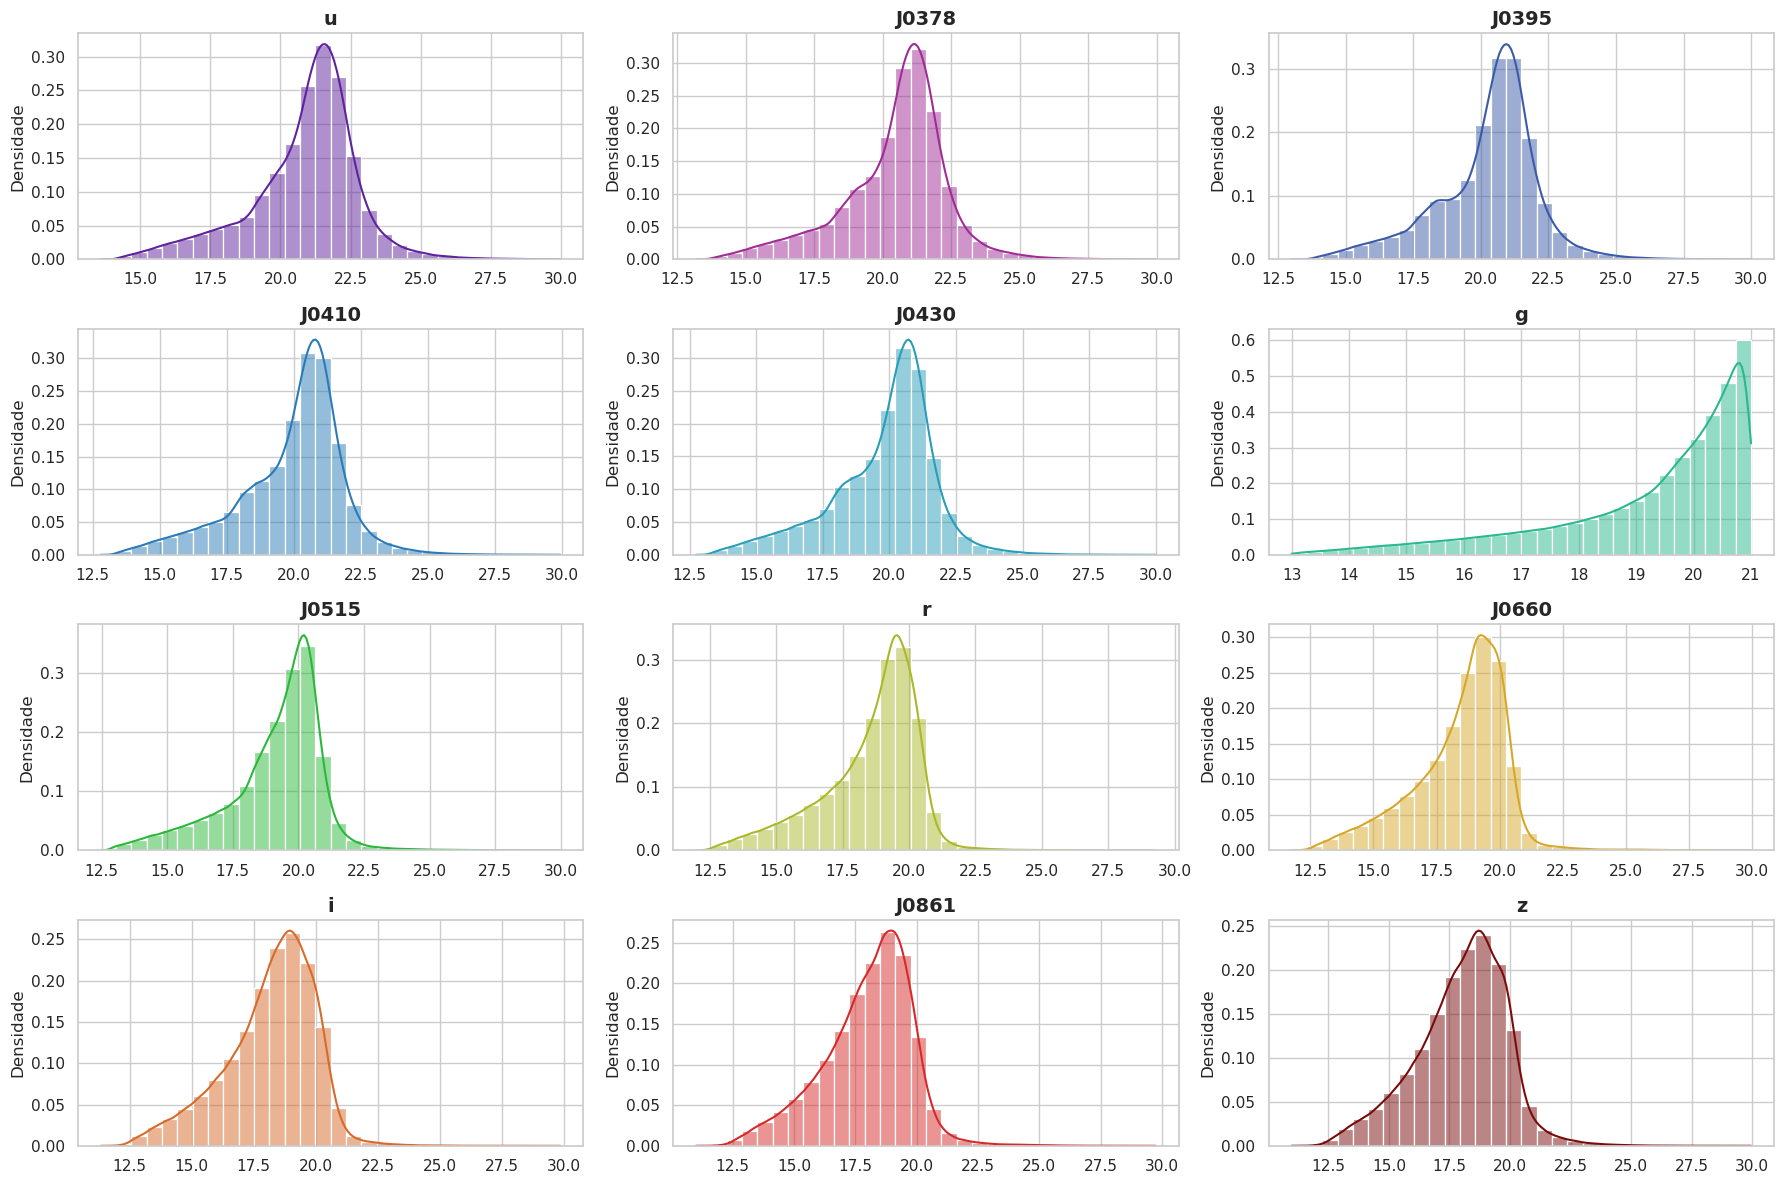
\includegraphics[width=1.0 \columnwidth,angle=0]{hist_distri_mags_data.png}
    \caption[]{Distribuições de densidade das magnitudes corrigidas para extinção nas 12 bandas fotométricas do S-PLUS (APER\_6) após a aplicação dos cortes de qualidade descritos. As bandas incluem 5 de banda larga ($u$, $g$, $r$, $i$, $z$) e 7 de banda estreita (J0378, J0395, J0410, J0430, J0515, J0660, J0861). Os cortes garantem a seleção de objetos com medições fotométricas confiáveis para a análise.}
    \label{fig:hist_distri_mags_data}
    \end{center}
\end{figure}
